\documentclass{article}
\usepackage{hyperref}
\usepackage{tikz}
\usepackage{python}
\usepackage[%
    natbib=true,%
    backend=biber,%
    backref=true,%
    citestyle=authoryear-comp,%
    bibstyle=authoryear,%
    maxbibnames=24,%
    maxcitenames=2,%
]{biblatex}

\hypersetup{%
    bookmarks=true,
    colorlinks=true,
    pdfauthor={Luis Pedro Coelho},
    citecolor=pondgreen,
    urlcolor=toastedchilipowder,
    linkcolor=toastedchilipowder,
}
\let\code\texttt
\addbibresource{references.bib}

\title{Jug: Software for Reproducible Computation}
\author{Luis Pedro Coelho}

\begin{document}
\maketitle

\section*{Abstract}
As computational pipelines become a bigger part of science, it is important to
ensure that the results are reproducible. All developed software should be able
to be run automatically without any user intervention.

In addition to being valuable to the wider community, which may wish to
reproduce or extend a published analysis, reproducible research practices allow
for better control over the project by the authors themselves. For example, if
necessary parameters to run a pipeline are kept separately from the code that
implements it (perhaps even in mind of the researcher), this leads to
error-prone analysis and opens up the possibility that when the results are to
be written up for publication, the researcher will no longer be able to even
completely describe the process that led to them.

For large projects, the use of multiple processors (either in the same machine
or distributed across a cluster) is necessary to obtain results in a useful
time frame. Furthermore, it is often the case that, as the project evolves, it
becomes necessary to save intermediate results while down-stream analyses are
designed (or redesigned) and implemented. Under many frameworks, this causes
having a single point of entry (often in the form of a single script or a
single main programme) for the computation becomes increasingly difficult.

Jug is a software framework which solves all of these problems in a simple way.
Jug supports caching of intermediate results, distribution of computation as
tasks across a network.

Jug is written in pure Python, is completely cross-platform, and available as
free software under the liberal MIT license. Jug is available from
\url{http://github.com/luispedro/jug}.
\bigskip
\bigskip

\section{Introduction}
The value of reproducible research in computational fields has been recognized
in several areas \citep{Vandewalle2009,Nordlie2009}. Although some of the
reports are still more forward looking rather than descriptive of current
practice, several implementations of reproducible papers (or executable papers)
have been proposed towards the goal of reproducing published analyses.

These solutions do not necessarily scale to large problems, those that take
several days, months, or years of CPU time. For very large problems,
specialized solutions are needed~\citep{mapReduce}. There is a range of
medium-sized problems that can be successfully tackled on a computer cluster
with a few hundred nodes or less (so that a computation that would take a
CPU-year can produce results in less than a day).

The typical ad hoc solution to this problem is to save intermediate files.
Often the design of the computation itself takes several iterations as
intermediate steps are improved. Thus, some intermediate results need to be
recomputed. This involves a great amount of human management of the state of
the computation, breaking it up into pieces, and issuing jobs on the cluster.

Jug is a task-based framework for Python, which supports saving and sharing of
intermediate results and parallelisation on computer clusters (or multi-core
machines).

By allowing caching of results, where the caching depends explicitly on the
input parameters of that computation. Any change in the parameters immediately
triggers a recomputation of all dependent results. The basic model is similar
to the one of the venerable Unix tool Make, which has been used before for
implementing reproducible research pipelines~\citep{Schwab00makingscientific}.

However, unlike make, jug is written in Python and tasks can consist of any
Python function and its arguments. This can include running external commands.
A jugfile (the file which specifies which tasks need to be run---named by
analogy to the makefiles of make) is a simple Python script with some added
notations (we will see just how little changes need to be made from a
conventional Python script).

\section{Design Choices}
\subsection{Task Based Architecture}

Jug is designed around tasks. A task is defined as a Python function and a set
of arguments, which may be Python values or the output of other tasks.

\begin{python}
from jug import Task

def count(imname):
    ...
    return value

def mean(args):
    return sum(args)/float(len(args))

images = glob('*.png')
counts = [Task(count, im) for im in images]
final = Task(mean, counts)
\end{python}

\begin{figure}
\begin{center}
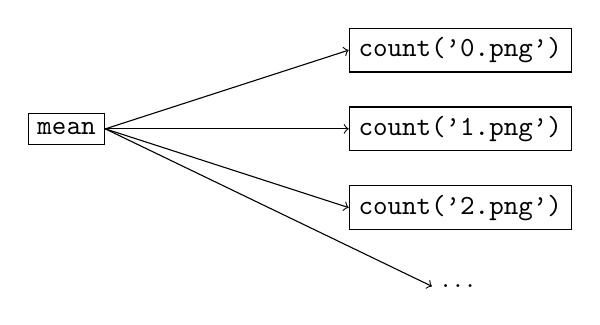
\begin{tikzpicture}
\node (mean) at (0,2) [draw] {\code{mean}};
\node (count0) at (5,3) [draw] {\code{count('0.png')}};
\node (count1) at (5,2) [draw] {\code{count('1.png')}};
\node (count2) at (5,1) [draw] {\code{count('2.png')}};
\node (countn) at (5,0) {\ldots};

\draw[->] (mean.east) -- (count0.west);
\draw[->] (mean.east) -- (count1.west);
\draw[->] (mean.east) -- (count2.west);
\draw[->] (mean.east) -- (countn.west);
\end{tikzpicture}

\end{center}
\caption{Simple Dependency Structure for Example in the Text. This assumes that
the directory had a collection of images names 0.png, 1.png,\ldots}
\label{fig:jug-deps}
\end{figure}

This code defines the task dependency structure represented in
Figure~\ref{fig:jug-deps}. As we can see, all of the \code{count} operations
can be run in parallel, while the \code{mean} operation must wait the result of
all of the other computation. The dependency structure is always a \textsc{dag}
(directed acyclic graph).

The code above has the construct \code{Task(f, args)} repeated several times.
Using the decorator \code{TaskGenerator} decorator this can be simplified to a
more natural syntax.

\begin{python}
from jug import TaskGenerator

@TaskGenerator
def count(imname):
    ...
    return value

@TaskGenerator
def mean(args):
    return sum(args)/float(len(args))

images = glob('*.png')
counts = map(count, images)
final = mean(counts)
\end{python}

As the reader can appreciate, this is identical to a traditional Python script,
except for the \code{@TaskGenerator} decorators. With a few limitations (which
unfortunately can give rise to complex error messages), scripts can be written
as if they were sequential Python scripts.

By default, jug looks for a file called \code{jugfile.py}, but any filename can
be used. Generically, we refer to the script being run as the jugfile.

\subsection{Jug subcommands}

Jug is structured as a series of subcommands, the most important of which are
\emph{execute}, \emph{status}, and \emph{shell}.

Execution is the command used for running the tasks. It performs a more complex
version of this loop:

\begin{python}
tasks = alltasks in topological sort order
while tasks:
    next = task.pop()
    if not next.has_run() and not next.is_running():
        while not next.can_run():
            wait a while
        with locked(next):
            next.run()
\end{python}

If run on a single processor, this will just run all of the tasks in order. It
is most interesting when it is run on multiple processors. There it executes
all of the tasks that can be executed in parallel.

Of course, the actual code is more complex than what is shown above,
particularly to make sure that the locking is performed correctly and that the
waiting step eventually times out (in order to handle the situation where
another process is hung).

\begin{figure}
\begin{verbatim}
$jug status images.py
Task name         Waiting      Ready   Finished    Running
----------------------------------------------------------
images.mean             1          0          0          0
images.count            0         20          0          0
..........................................................
Total:                  1         20          0          0
\end{verbatim}
\caption{Output of \code{jug status}. The \texttt{\$} sign shown is the command
line prompt, and the status subcommand was run. At this point, nothing has been
run. The output has been edited for space reasons (spacing columns were
removed).}
\label{fig:jug-status-output}
\end{figure}

The status command prints out a summary of the status of all of the tasks.
Figure~\ref{fig:jug-status-output} shows the output of this command using the
example jugfile above. We assume that the jugfile was called \code{images.py}
on disk and that there were 20~images in the directory. We can see that there
are 20~tasks ready to run, while the \code{mean} task is still waiting for the
results of the other tasks.

\subsection{Backends}

A basic feature of jug is its ability to save and load results. Each task
\code{Task(f, args)} is represented by a hash of \code{f} and \code{args} in a
way that uniquely identifies it.

A jug backend must then support four basic operations:

\begin{description}
\item[save] Saving a Python object by its hash name.
\item[load] Loading a Python object by its hash name.
\item[lock] Creating a lock by hash name. Naturally, this lock must be created
atomically.
\item[release] Releasing the lock.
\end{description}

A few other operations, such as deletion and listing of names are also
supported.

The filesystem can support all of the above operations if the backend is coded
correctly to avoid race conditions. This is the default backend, identified
simply by a directory name. Inside this directory, files named by a hexadecimal
representation of their hashes. Objects are saved using Python's \code{pickle}
module with zlib compression. As a special case, \code{numpy} arrays
\citep{numpy} are saved to disk directly. For functionality, there was no need
for this inelegant special case as \code{numpy} can be saved as a pickle dump,
but \code{numpy} arrays are a very common data type in scientific programming
and saving them directly allows for very fast saving and loading (they are
represented on disk as a header followed by the binary information they
contain).

Another backend currently included with jug is a redis backend. Redis a
name-key database system.\footnote{See the redis webpage, at
\href{http://redis.io}{redis.io}, for detailed information about redis.} Redis
is particularly recommended for the case where there are many small objects
being saved. In this case, keeping each as a separate file on disk would incur
a large space penalty, while redis keeps them all in the same file.

Finally, there is an in-memory backend. This was initially developed for
testing, but can be useful on its own.

\subsection{Asynchronous Function}

Parallelisation is achieved by running more than one jug process
simultaneously. All of the synchronisation is outsourced to the backend. As
long as all of the processes can access the backend, there is no need for them
to communicate directly. It can even be the case that processors start working
on tasks in mid-processing. This makes jug usable in batch-based computer
cluster environments, which are quite common in research institutions.

\subsection{Software Development With Jug}

The output of computation can be obtained from jug in two ways: (1) One can
simply write a task that writes to a file in the desired format. (2) They can
be inspected interactively using the \emph{shell} subcommand. It is expected
that the first option will be used for the final version of the computation,
whilst the second one is most helpful during development.

The shell subcommand, invokes an IPython instance with all the objects in the
jugfile loaded. IPython is an enhanced interactive shell for Python
\citep{Perez2007}. A few functions are added to the namespace, in particular,
\code{value} can load the results of a task object if necessary.

\begin{figure}
\begin{center}
\begin{verbatim}
$jug shell images.py

=========
Jug Shell
=========


Available jug functions:
    - value() : loads a specific object
    - load_all() : loads all objects

Enjoy...


In [1]: value(final)
Out[1]: 7.5

In [2]: value(counts)
Out[2]: [7, 7, 7, 7, 7, ... 8, 8, 8, 8, 8, 8, 8, 8, 8]
\end{verbatim}
\end{center}
\caption{Interaction with \code{jug shell}. The \code{value} function loads and
returns the result from any task. The final line has been edited (marked with
\ldots) for presentation purposes.}
\label{fig:jug-shell-interaction}
\end{figure}

Figure~\ref{fig:jug-shell-interaction} shows a possible interaction session
with jug shell. While having to explicitly load all the results is a bit
bothersome, it can be better than pre-loading all of them. It is much faster at
startup. Consider too that the user might not load more than a few objects. In
some cases, loading all of the objects simultaneously might even be impossible
due to memory constraints. Further, this allows exploration of the task
structure for debugging.

This is a feature which can be used to debug one's own code or to explore the
results of a computation by others.

\subsection{Result Invalidation}

It is often the case that one improves a step in a computational pipeline and
wished to obtain the result of recomputing the pipeline while reusing as much
of the previously computed intermediate results. Before using Jug, I found this
to be a very error-prone operation: by not removing enough of the intermediate
files, it was easy to generate an irreproducible state where part of the
computations were made using one version of the code and part with another.

Therefore, jug adds some support for result invalidation. When a results from a
task are invalidated, all tasks which, directly or indirectly, depend on them
are also marked for deletion.

It is still necessary to manually invalidate tasks. An alternative, which I
considered, was to have the code which implements the task be taken into
account while computing the hash. While this would add another layer of
protection, it would still be possible to make mistakes. If the function
depended on other functions, especially if this was done in a dynamic way, it
could be hard to discover all dependencies (cf.\ sumatra~\footnote{Sumatra is a
tool to collect all dependencies that are necessary to run a particular
computation. Its webpage is located at
\url{http://neuralensemble.org/trac/sumatra}.}). Additionally, even minute
refactoring of the code would lead to over eager recomputation. This could make
the developer wary of making improvements in their code, resulting in overall
worse code.

Therefore, I chose to force the user to explicitly invalidate his results,
while supporting automatic dependency discovery to make it easier for the user.
The recommendation is still that the user run the full pipeline from start to
finish once they are satisfied with the state of the code and certainly before
publication, but the pipeline development stage can be more agile.

\section{Methods}
\section{Example}
I will present an example from my research. Although it introduces some
unnecessary complexity, it has the advantage of being a real-life example of
the usage of jug.

The goal of this project was to demonstrate that using local features, in
particular speeded-up robust features (henceforth,
\textsc{surf})~\cite{surf-paper} improves over image-global features for
classification of microscope images. A variation of standard \textsc{surf},
\textsc{surf}-ref, was introduced and tested.

To evaluate classification, the dataset is broken up into 10~pieces and each of
the pieces is held-out of the analysis and then used to evaluate analysis (the
final result is the average of all ten values). This is known as
cross-validation. In this case, I use another library (which I also wrote)
which has a built-in method for jug-aware cross-validation.

\begin{python}
from jug import TaskGenerator, CachedFunction

# pyslic is used for subcellular location analysis
import pyslic

# milk (machine learning toolkit)
from milk.ext.jugparallel import nfoldcrossvalidation

datasets = [ 'data0', 'data1', ]
featuresets = [ 'field-dna+', 'surf', 'surf-ref', ]

def load(dset):
    '''
    This function assumes that the images are stored in
    ../data/dset with filenames matching the pattern
    label-(protein|dna)-([0-9]).tiff
    '''
    from os import listdir
    images = []
    base = '../data/'+dset
    for path in listdir(base):
        if not 'protein' in path: continue
        label = path.split('-')[0]
        # We only store paths and will load data on demand
        # This save memory.
        im = pyslic.Image({
                'protein': base + path,
                'dna' : base + path.replace('protein','dna')
                })
        im.label = label
        images.append(im)
    return images

# pyslic.computefeatures takes an image and an identifier of the
# feature set and returns a set of features (as a numeric array).
#
# TaskGenerator can be used directly to adapt existing functions
computefeatures = TaskGenerator(pyslic.computefeatures)

# or it can be used as a decorator on a newly defined function
@TaskGenerator
def output(cmatrix, dset, fset):
    output = file('results/cmatrix-'+dset+'-'+fset+'.txt', 'w')
    print >>output, cmatrix
    output.close()

features = []
for dset in datasets:
    images = CachedFunction(load, dset)
    labels = [im.label for im in images]
    for fset in featuresets:
        features = [computefeatures(im, fset) for im in images]
        cmatrix = nfoldcrossvalidation(features, labels)
        output(cmatrix, dset, fset)
\end{python}

Figure~\ref{fig:jug-deps-complex} shows the dependency structure of this
examples. The main feature is the fan-out/fan-in which is associated with
map-reduce frameworks.

\begin{figure}
\begin{center}
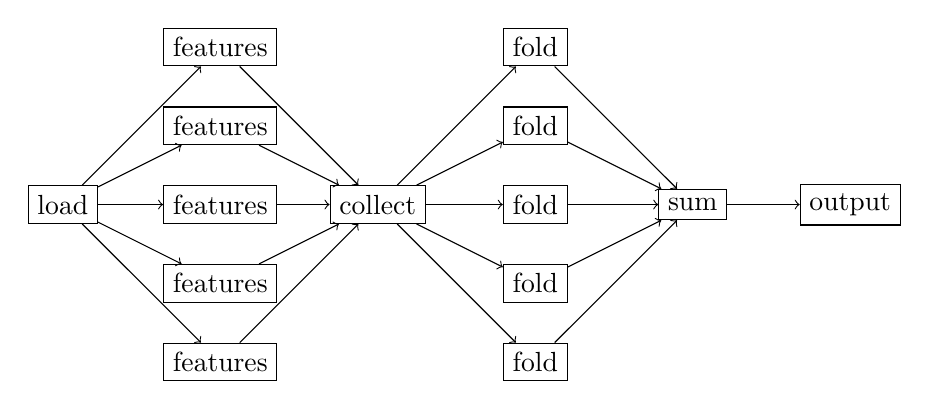
\begin{tikzpicture}
\node (load) at (0,0) [draw] {load};
\node (collect) at (4,0) [draw] {collect};
\node (sum) at (8,0) [draw] {sum};
\node (output) at (10,0) [draw] {output};

\path[->]
    (sum) edge (output);

\foreach \y in {-2,-1,0,1,2} {%
    \node (features\y) at (2,\y) [draw] {features};
    \path[->]
        (load) edge (features\y)
        (features\y) edge (collect);
}

\foreach \y in {-2,-1,0,1,2} {%
    \node (fold\y) at (6,\y) [draw] {fold};
    \path[->]
        (collect) edge (fold\y)
        (fold\y) edge (sum);
}
\end{tikzpicture}

\end{center}
\caption{Dependency Structure for second example in the Text. The
fan-out/fan-in structure is typical (it is an instance of the map-reduce
framework).}
\label{fig:jug-deps-complex}
\end{figure}

\section{Development of Jug}
Jug is available under the MIT software license, which grants the user right to
use, copy, and modify the code almost at will. It is developed using the git
version control tool, with the project being hosted on the github
platform.\footnote{The jug project is available at
\url{https://www.github.com/luispedro/jug}.} An open mailing-list provides
support and reported bugs are generally fixed within hours.

Jug includes a full test suite. There are no known bugs.

Jug has been available in the Python Package Index\footnote{The Python Package
Index, PyPI, is accessible at \url{http://pypi.python.org}.} since May~2009
through June~2012 and has been downloaded over 13,000~times (some of these
downloads may, of course, represent upgrades, and users which downloaded it
from some other source will not be counted).

\section{Discussion}

\subsection{Similar Tools}

\citet{Fomel2007} proposed a system built on top of Scons which shared
superficially similar design. Scons, like Make, is a build system. It supports
spawning parallel jobs using multiple threads. In the original use case, the
tasks are delegated to other commands and the operating system can take care of
parallelism. If, however, the tasks are computationally intensive in Python,
contention for the global interpreter lock will limit the amount of real
parallelism.\footnote{In the most commonly used Python interpreters, there is a
lock that prevents more than one thread from simultaneously executing
interpreted code, although they can execute non-interpreted code, as calling an
external programme or certain external libraries.} Ruffus is another
Python-based solution which supports parallel execution of pipelines
\citep{Goodstadt16092010}. There is a strong dependency on the filesystem,
which makes its use very different from jug usage, which strives to make its
usage similar to straight Python usage. Using the Ruby programming language,
\citet{mishima2011} proposed Pwrake, which supports parallel execution of
bioinformatics workflows written (or accessible) in that language.

Of interest, is also the \textsc{IncPy} implementation of a Python interpreter
with automatic persistent memoization~\cite{Guo_IncPy,Guo_IncPy_pre}. The
arguments made for that system apply to Jug as well, with a few differences.
Their system implements automatic memoization, while, using Jug, the user needs
to automatically annotate functions to memoize using \texttt{TaskGenerator}.
This extra control can be necessary to avoid a proliferation of intermediate
results when these are very large (often a very large intermediate output is
not necessary, and only a summary must be kept). Additionally, Jug supports
running tasks in parallel, a functionality that is absent from \textsc{IncPy}.

\subsection{Conclusions}

Unlike most previous tools for reproducible research, jug focuses on the
development of the computation as much as its communication. In fact, when it
comes to communication other tools might be better suited as they combine
written exposition with computer code. They can be used in combination with jug
as they do not often provide caching and distribution, needed for large
projects. While the simplest mode of jug use is to have a single
\textit{jugfile}, a jugfile can import the results of another. For example, a
first jugfile might perform all heavy-duty computation and be run on a
computing cluster. A second script could be embedded inside an executable paper
to generate tables and plots \citep{Delescluse2011}. This faster script could
be run as part of building the paper (while the longer script would take too
long).

While it still possible to make errors (for example, by changing the code but
neglecting to invalidate the results), jug improves the pipeline development
experience and makes the programming researcher more productive and less
error-prone.

Jug was not designed to compete with complete map/reduce frameworks such as
Hadoop, which scale better to very large projects. However, those frameworks
have much higher costs in terms of development time (code must be written
especially for the framework) and overhead (starting up and shutting down jobs
can take much longer and using non-Java code has additional computational
costs). For scientists using small to medium-sized cluster (hundreds, not
thousands, of nodes), with a shared file-system (as opposed to the distributed
file-systems necessary for truly large amounts of data) jug might provide a
better trade-off than those higher-powered alternatives.

In the last few years, I have not undertaken any computational research project
without the use of jug to manage my computations. Additionally, I (and my
co-authors) have made the resulting results directories available\footnote{See
the links at
\url{http://murphylab.cbi.cmu.edu/software/software_from_papers.html}}. The
tool has become an indispensible part of my toolkit.

\printbibliography
\end{document}
